% 4_algoritmo.tex

% Un diagrama de flujo del algoritmo de la solución propuesta.
\section{Algoritmo propuesto}

Para implementar el comportamiento deseado, se propone utilizar los algoritmos mostrados en las Figuras \ref{fig:flowchart-tx} y \ref{fig:flowchart-rx}.
A diferencia de un diseño simétrico, en esta solución cada dispositivo tiene un rol fijo: uno actúa exclusivamente como transmisor y el otro exclusivamente como receptor.

El nodo transmisor, cuyo flujo se ilustra en la Figura \ref{fig:flowchart-tx}, permanece en espera hasta que el usuario presiona el botón de inicio.
Al detectarse dicha pulsación, el dispositivo realiza la grabación y transmisión del audio.
Al finalizar, el nodo regresa al estado de espera, listo para una nueva transmisión.

\begin{figure}[htb]
    \centering
    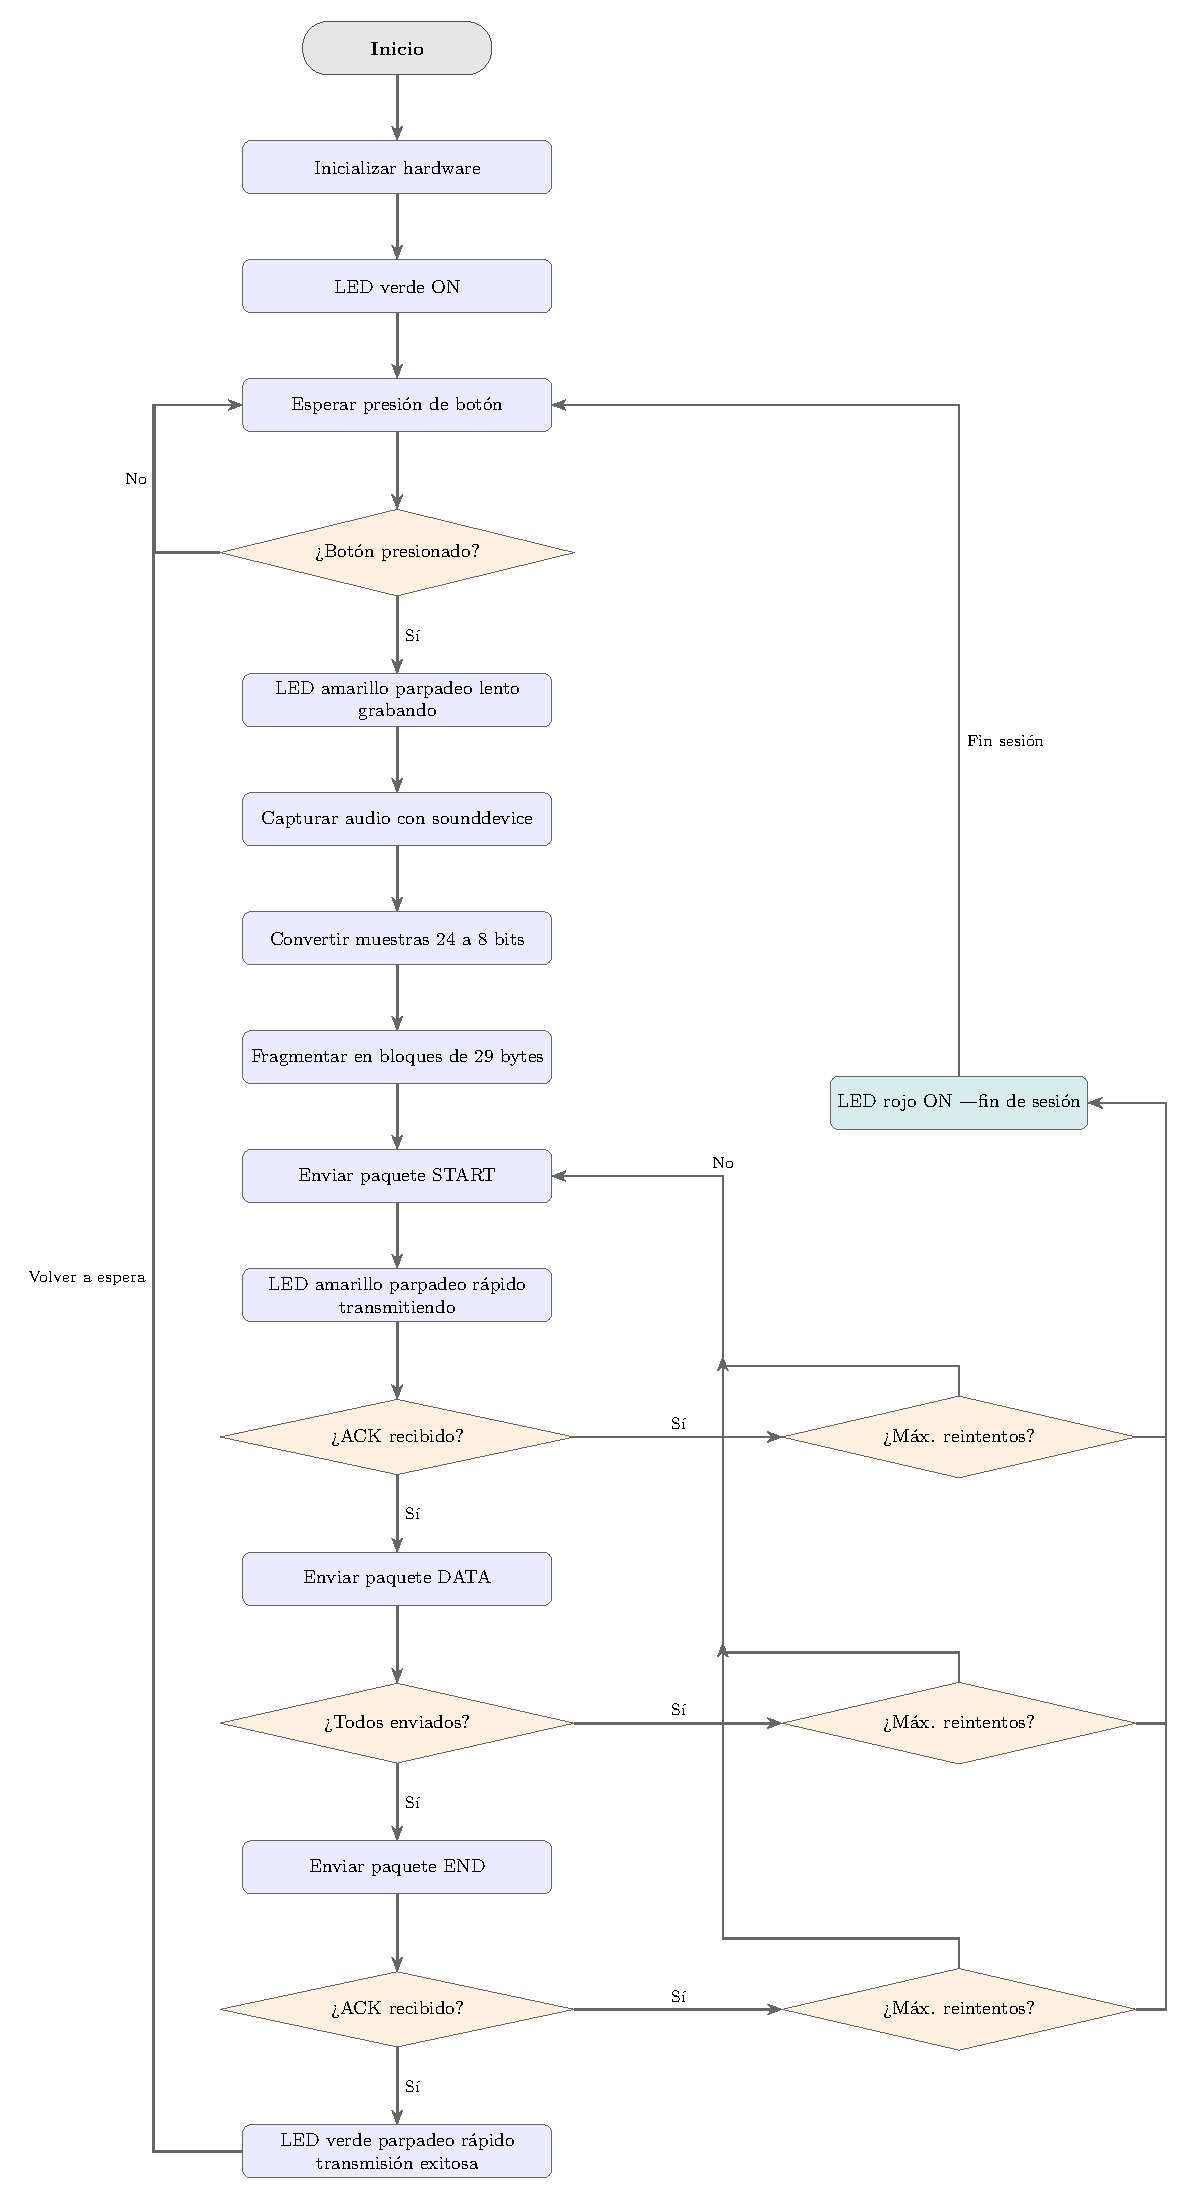
\includegraphics[width=1\columnwidth]{images/fc_tx.pdf}
    \caption{Diagrama de flujo del nodo transmisor.}
    \label{fig:flowchart-tx}
\end{figure}

El nodo receptor, por su parte, permanece continuamente en modo de recepción a la espera de un \texttt{START} que señale el inicio de una transmisión (este diseño se especifica en la sección \ref{sec:organizacion_transferencia}).
Al recibirlo, gestiona la recepción y reproducción del audio, como se ilustra en la Figura \ref{fig:flowchart-rx}.
Una vez finalizado, el nodo regresa al estado de espera para atender una nueva transmisión.

\begin{figure}[htb]
    \centering
    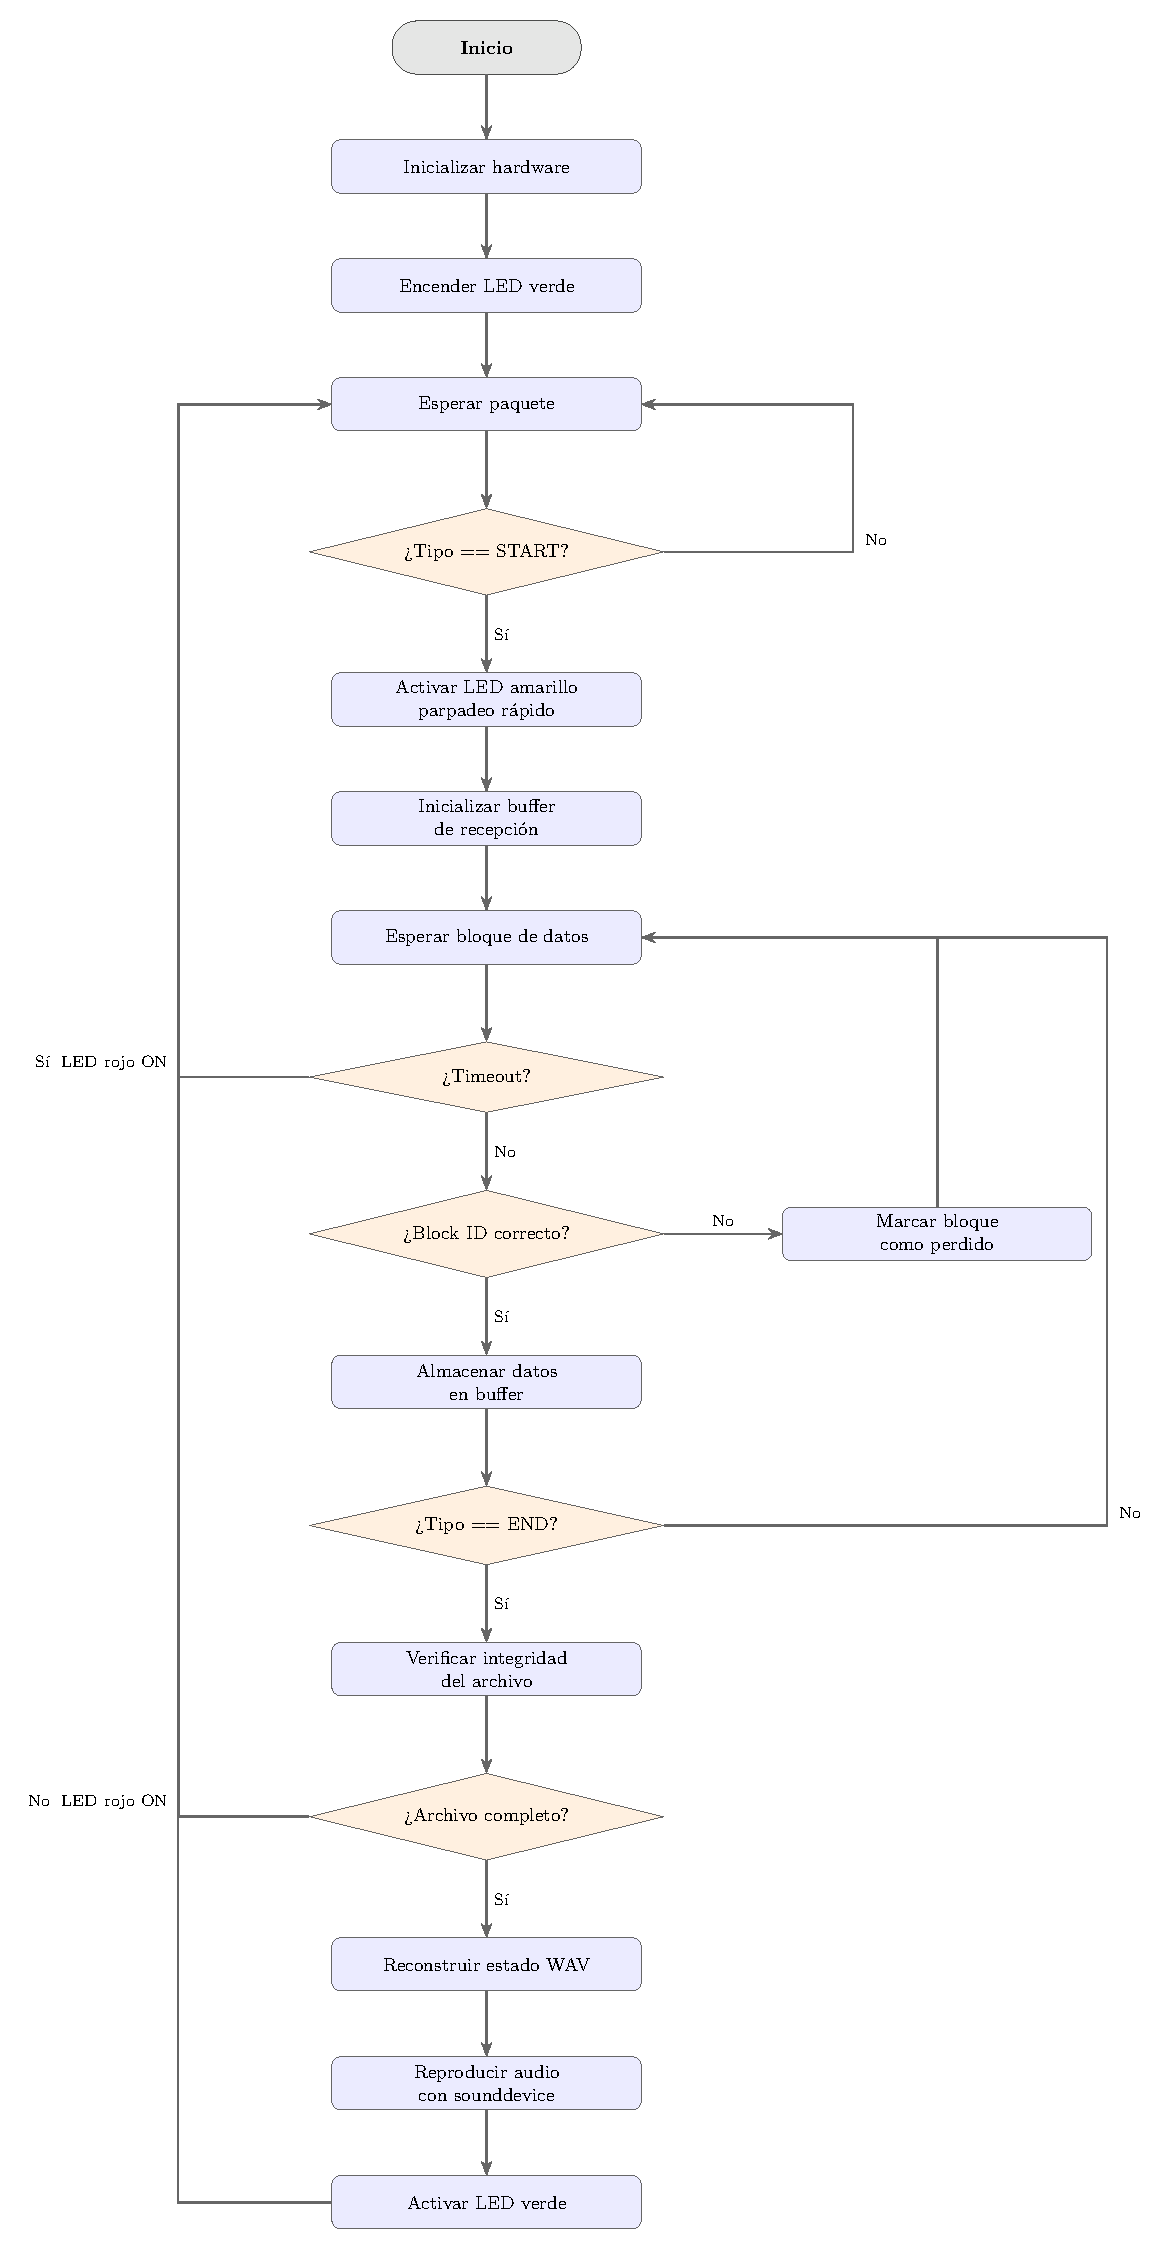
\includegraphics[width=1\columnwidth]{images/fc_rx.pdf}
    \caption{Diagrama de flujo del nodo receptor.}
    \label{fig:flowchart-rx}
\end{figure}

Por simplicidad, no se considerará el caso en que el botón de transmisión se presione durante un proceso de transmisión o reproducción en curso.
Se asume que el botón únicamente se acciona una vez transcurrido un tiempo suficiente para completar el proceso anterior.
De no cumplirse esta condición, no se garantiza el funcionamiento correcto del sistema.

La comunicación inalámbrica entre dispositivos se realizará mediante el protocolo \textit{Enhanced ShockBurst} (ESB), que se detalla en la siguiente sección.

Se usarán tres LEDs para indicar al usuario el estado del sistema durante la captura, transmisión, recepción y reproducción según el código mostrado en el Cuadro \ref{tab:led_states}.

\begin{table}[htb]
\centering
\begin{tabular}{lccc}
\toprule
Estado & LED verde & LED amarillo & LED rojo \\
\midrule
Listo / espera      & Encendido & Apagado        & Apagado   \\
Grabando            & Apagado   & Parpadeo lento & Apagado   \\
Transmitiendo       & Apagado   & Parpadeo rápido & Apagado  \\
Recibiendo          & Apagado   & Parpadeo rápido & Apagado  \\
Reintentando paquete & Apagado  & Encendido      & Parpadeo  \\
Error               & Apagado   & Apagado        & Encendido \\
Transmisión exitosa & Parpadeo rápido & Apagado   & Apagado   \\
Reproduciendo       & Encendido & Encendido      & Apagado   \\
\bottomrule
\end{tabular}
\caption{Estados de los LEDs.}
\label{tab:led_states}
\end{table}

Como alternativa de diseño, una forma más elegante de resolver el presente problema es a partir de una máquina de estados finita tanto para el nodo transmisor como el receptor.
En las Figuras \ref{fig:fsm_tx} y \ref{fig:fsm_rx} se muestran los diagramas de estados planteados para cada una, respectivamente.
Este diseño permite modelar el comportamiento del hardware utilizado de forma sencilla y facilita la programación y \textit{debugging}, en comparación con una lógica condicional extensa.
Por lo que, se valorará su implementación en la siguiente etapa del proyecto.
Entonces, los diagramas de flujo mostrados anteriormente permiten entender el comportamiento requerido y con los diagramas de estados se resume el planteamiento ideado a nivel de código.

\begin{figure}[htb]
    \centering
    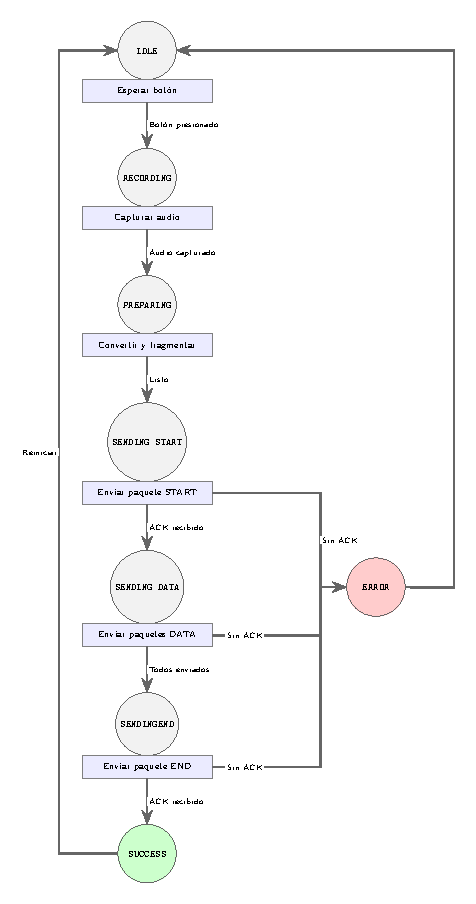
\includegraphics[width=\columnwidth]{images/fsm_tx.pdf}
    \caption{Diagrama de estados del nodo transmisor.}
    \label{fig:fsm_tx}
\end{figure}

\begin{figure}[htb]
    \centering
    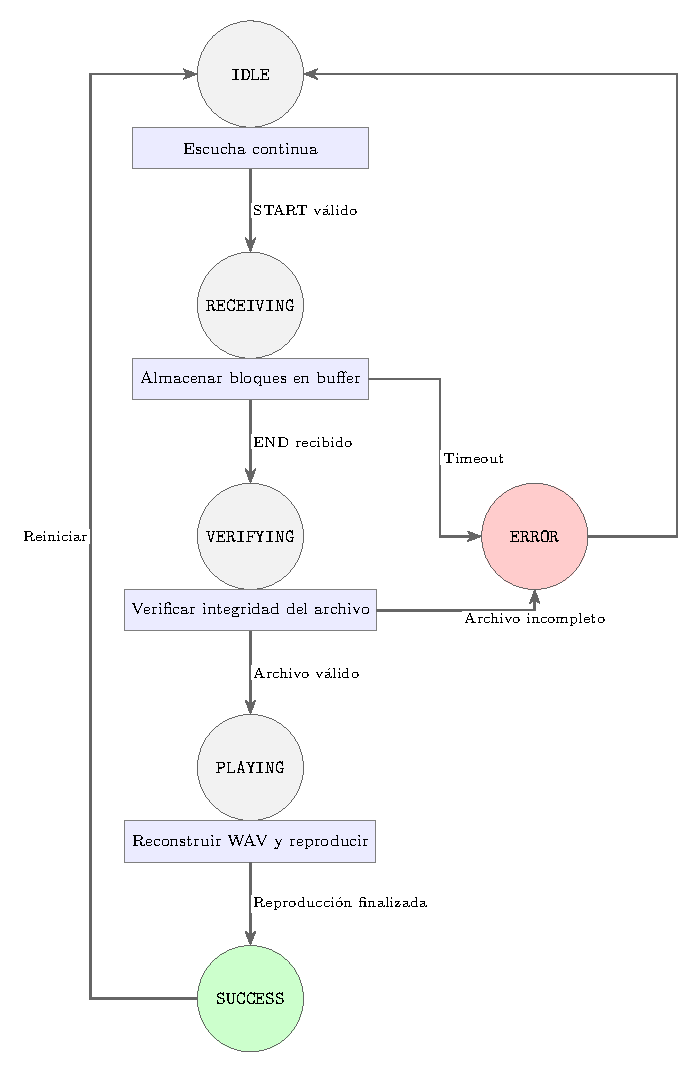
\includegraphics[width=\columnwidth]{images/fsm_rx.pdf}
    \caption{Diagrama de estados del nodo receptor.}
    \label{fig:fsm_rx}
\end{figure}


% PRUEBAS
% % ----------------------------------------------
% \begin{figure}[htb]
% \centering
% \begin{adjustbox}{width=\columnwidth}
% \begin{tikzpicture}[
%     state/.style={circle, draw=black, fill=gray!10,
%                   minimum size=1.8cm, font=\small\ttfamily,
%                   text centered},
%     action/.style={rectangle, draw=black, fill=blue!8,
%                    minimum width=3.5cm, minimum height=0.6cm,
%                    font=\footnotesize, text centered},
%     arrow/.style={->, >=stealth, thick},
%     label/.style={font=\scriptsize, midway, fill=white, inner sep=1pt}
% ]

% % Estados
% \node[state]             (idle)    at (0, 0)    {IDLE};
% \node[action]            (a_idle)  at (0, -1.8) {Esperar botón};
% \node[state]             (rec)     at (0, -4)   {RECORDING};
% \node[action]            (a_rec)   at (0, -5.8) {Capturar audio};
% \node[state]             (prep)    at (0, -8)   {PREPARING};
% \node[action]            (a_prep)  at (0, -9.8) {Convertir y fragmentar en bloques};
% \node[state]             (start)   at (0, -12)  {SENDING START};
% \node[action]            (a_start) at (0, -13.8){Enviar paquete \texttt{START}};
% \node[state]             (data)    at (0, -16)  {SENDING DATA};
% \node[action]            (a_data)  at (0, -17.8){Enviar paquetes \texttt{DATA}};
% \node[state]             (end)     at (0, -20)  {SENDING END};
% \node[action]            (a_end)   at (0, -21.8){Enviar paquete \texttt{END}};
% \node[state, fill=green!20] (success) at (0, -24)  {SUCCESS};
% \node[state, fill=red!20]   (error)   at (6, -16)  {ERROR};

% % Flujo principal
% \draw[arrow] (idle)    -- (a_idle);
% \draw[arrow] (a_idle)  -- node[label, right] {Botón presionado} (rec);
% \draw[arrow] (rec)     -- (a_rec);
% \draw[arrow] (a_rec)   -- node[label, right] {Audio capturado}  (prep);
% \draw[arrow] (prep)    -- (a_prep);
% \draw[arrow] (a_prep)  -- node[label, right] {Listo}            (start);
% \draw[arrow] (start)   -- (a_start);
% \draw[arrow] (a_start) -- node[label, right] {ACK recibido}     (data);
% \draw[arrow] (data)    -- (a_data);
% \draw[arrow] (a_data)  -- node[label, right] {Todos enviados}   (end);
% \draw[arrow] (end)     -- (a_end);
% \draw[arrow] (a_end)   -- node[label, right] {ACK recibido}     (success);

% % Retorno a IDLE desde SUCCESS
% \draw[arrow] (success) to[bend right=70] node[label, left] {Timeout} (idle);

% % Transiciones de error
% \draw[arrow] (a_start) -- node[label, above] {Sin ACK} (error);
% \draw[arrow] (a_data)  -- node[label, above] {Sin ACK} (error);
% \draw[arrow] (a_end)   to[bend left=20] node[label, above] {Sin ACK} (error);
% \draw[arrow] (error)   to[bend left=20] node[label, right] {Timeout} (idle);

% \end{tikzpicture}
% \end{adjustbox}
% \caption{Máquina de estados del nodo transmisor.}
% \label{fig:fsm_tx}
% \end{figure}

% \begin{figure}[htb]
% \centering
% \begin{adjustbox}{width=\columnwidth}
% \begin{tikzpicture}[
%     state/.style={circle, draw=black, fill=gray!10,
%                   minimum size=1.8cm, font=\small\ttfamily,
%                   text centered},
%     action/.style={rectangle, draw=black, fill=blue!8,
%                    minimum width=3.5cm, minimum height=0.6cm,
%                    font=\footnotesize, text centered},
%     arrow/.style={->, >=stealth, thick},
%     label/.style={font=\scriptsize, midway, fill=white, inner sep=1pt}
% ]

% % Estados
% \node[state]             (idle)     at (0, 0)    {IDLE};
% \node[action]            (a_idle)   at (0, -1.8) {Escucha continua};
% \node[state]             (recv)     at (0, -4)   {RECEIVING};
% \node[action]            (a_recv)   at (0, -5.8) {Almacenar bloques en buffer};
% \node[state]             (verify)   at (0, -8)   {VERIFYING};
% \node[action]            (a_verify) at (0, -9.8) {Verificar integridad del archivo};
% \node[state]             (play)     at (0, -12)  {PLAYING};
% \node[action]            (a_play)   at (0, -13.8){Reconstruir WAV y reproducir};
% \node[state, fill=green!20] (success) at (0, -16)  {SUCCESS};
% \node[state, fill=red!20]   (error)   at (6, -8)   {ERROR};

% % Flujo principal
% \draw[arrow] (idle)     -- (a_idle);
% \draw[arrow] (a_idle)   -- node[label, right] {\texttt{START} válido}      (recv);
% \draw[arrow] (recv)     -- (a_recv);
% \draw[arrow] (a_recv)   -- node[label, right] {\texttt{END} recibido}      (verify);
% \draw[arrow] (verify)   -- (a_verify);
% \draw[arrow] (a_verify) -- node[label, right] {Archivo válido}             (play);
% \draw[arrow] (play)     -- (a_play);
% \draw[arrow] (a_play)   -- node[label, right] {Reproducción finalizada}    (success);

% % Retorno a IDLE desde SUCCESS
% \draw[arrow] (success) to[bend right=70] node[label, left] {Timeout} (idle);

% % Paquete desconocido loop
% \draw[arrow] (a_idle) to[loop right] node[label, right] {Paquete desconocido} (a_idle);

% % Botón presionado en RECEIVING
% \draw[arrow] (recv) to[bend right=60] node[label, left] {Botón presionado} (idle);

% % Timeout en RECEIVING
% \draw[arrow] (a_recv) to[bend left=30] node[label, above] {Timeout} (verify);

% % Error
% \draw[arrow] (a_verify) -- node[label, above] {Archivo inválido} (error);
% \draw[arrow] (error)    to[bend left=20] node[label, right] {Timeout} (idle);

% \end{tikzpicture}
% \end{adjustbox}
% \caption{Máquina de estados del nodo receptor.}
% \label{fig:fsm_rx}
% \end{figure}

% \begin{figure}[htb]
% \centering
% \begin{adjustbox}{width=\columnwidth}
% \begin{tikzpicture}[
%     block/.style={rectangle, rounded corners, draw=black, fill=gray!10,
%                   minimum width=4cm, minimum height=0.7cm,
%                   text centered, font=\small},
%     decision/.style={diamond, draw=black, fill=yellow!15,
%                      minimum width=3cm, minimum height=0.7cm,
%                      text centered, font=\small, aspect=2},
%     arrow/.style={->, >=stealth, thick},
%     label/.style={font=\footnotesize}
% ]

% \node[block]    (init)    at (0,0)     {Inicializar hardware};
% \node[block]    (idle)    at (0,-1.5)  {LED verde ON $\rightarrow$ estado listo};
% \node[block]    (wait)    at (0,-3)    {Esperar presi\'on de bot\'on};
% \node[block]    (rec)     at (0,-4.5)  {LED amarillo parpadeo lento $\rightarrow$ grabando};
% \node[block]    (cap)     at (0,-6)    {Capturar audio con \texttt{sounddevice}};
% \node[block]    (conv)    at (0,-7.5)  {Convertir muestras de 24 a 8 bits con \texttt{numpy}};
% \node[block]    (frag)    at (0,-9)    {Fragmentar en bloques de 29 bytes};
% \node[block]    (sstart)  at (0,-10.5) {Enviar paquete \texttt{START}};
% \node[block]    (txled)   at (0,-12)   {LED amarillo parpadeo r\'apido $\rightarrow$ transmitiendo};
% \node[decision] (ack1)    at (0,-13.8) {ACK recibido?};
% \node[decision] (maxret)  at (5,-13.8) {M\'ax. reintentos?};
% \node[block]    (sdata)   at (0,-16)   {Enviar paquete \texttt{DATA}};
% \node[decision] (allsent) at (0,-17.8) {Todos enviados?};
% \node[decision] (ack2)    at (5,-17.8) {M\'ax. reintentos?};
% \node[block]    (send)    at (0,-20)   {Enviar paquete \texttt{END}};
% \node[decision] (ack3)    at (0,-21.8) {ACK recibido?};
% \node[decision] (ack3ret) at (5,-21.8) {M\'ax. reintentos?};
% \node[block, fill=green!15] (success) at (0,-24) {LED verde parpadeo r\'apido $\rightarrow$ \'exito};
% \node[block, fill=red!15]   (error)   at (9,-13.8) {LED rojo ON $\rightarrow$ fin sesi\'on};

% % Flujo principal
% \draw[arrow] (0,1) -- node[label, right] {INICIO} (init);
% \draw[arrow] (init)    -- (idle);
% \draw[arrow] (idle)    -- (wait);
% \draw[arrow] (wait)    -- (rec);
% \draw[arrow] (rec)     -- (cap);
% \draw[arrow] (cap)     -- (conv);
% \draw[arrow] (conv)    -- (frag);
% \draw[arrow] (frag)    -- (sstart);
% \draw[arrow] (sstart)  -- (txled);
% \draw[arrow] (txled)   -- (ack1);
% \draw[arrow] (ack1)    -- node[label, right] {S\'i} (sdata);
% \draw[arrow] (sdata)   -- (allsent);
% \draw[arrow] (allsent) -- node[label, right] {S\'i} (send);
% \draw[arrow] (send)    -- (ack3);
% \draw[arrow] (ack3)    -- node[label, right] {S\'i} (success);
% \draw[arrow] (success) to[bend right=80] node[label, left] {Volver a espera} (wait);

% % Reintentos START
% \draw[arrow] (ack1)   -- node[label, above] {No} (maxret);
% \draw[arrow] (maxret) -- node[label, above] {S\'i} (error);
% \draw[arrow] (maxret) to[bend left=30] node[label, right] {No $\rightarrow$ reintentar} (sstart);
% \draw[arrow] (error)  to[bend left=20] node[label, above] {Fin sesi\'on} (wait);

% % Reintentos DATA
% \draw[arrow] (allsent) -- node[label, above] {No $\rightarrow$ continuar} (ack2);
% \draw[arrow] (ack2)    -- node[label, above] {S\'i} (error);
% \draw[arrow] (ack2)    to[bend left=30] node[label, right] {No $\rightarrow$ reintentar} (sdata);

% % Reintentos END
% \draw[arrow] (ack3)    -- node[label, above] {No} (ack3ret);
% \draw[arrow] (ack3ret) -- node[label, above] {S\'i} (error);
% \draw[arrow] (ack3ret) to[bend left=30] node[label, right] {No $\rightarrow$ reintentar} (send);

% \end{tikzpicture}
% \end{adjustbox}
% \caption{Diagrama de flujo del nodo transmisor.}
% \label{fig:flow_tx}
% \end{figure}

% \begin{figure}[htb]
% \centering
% \begin{adjustbox}{width=\columnwidth}
% \begin{tikzpicture}[
%     block/.style={rectangle, rounded corners, draw=black, fill=gray!10,
%                   minimum width=4cm, minimum height=0.7cm,
%                   text centered, font=\small},
%     decision/.style={diamond, draw=black, fill=yellow!15,
%                      minimum width=3cm, minimum height=0.7cm,
%                      text centered, font=\small, aspect=2},
%     arrow/.style={->, >=stealth, thick},
%     label/.style={font=\footnotesize}
% ]

% \node[block]    (init)    at (0,0)     {Inicializar hardware};
% \node[block]    (idle)    at (0,-1.5)  {LED verde ON $\rightarrow$ estado espera};
% \node[block]    (listen)  at (0,-3)    {Modo escucha continua};
% \node[decision] (pkt)     at (0,-4.8)  {Paquete recibido?};
% \node[decision] (isstart) at (0,-7)    {Tipo == \texttt{START}?};
% \node[block]    (prepbuf) at (0,-8.8)  {LED amarillo parpadeo r\'apido};
% \node[block]    (buf)     at (0,-10.3) {Preparar buffer con par\'ametros de \texttt{START}};
% \node[block]    (waitpkt) at (0,-11.8) {Esperar paquete};
% \node[decision] (pkt2)    at (0,-13.6) {Paquete recibido?};
% \node[decision] (timeout) at (5,-13.6) {Timeout?};
% \node[decision] (blknum)  at (0,-15.8) {N\'um. bloque correcto?};
% \node[block]    (mark)    at (5,-15.8) {Marcar bloque como perdido};
% \node[block]    (store)   at (0,-17.3) {Almacenar bloque en buffer};
% \node[decision] (isend)   at (0,-19.1) {Tipo == \texttt{END}?};
% \node[block]    (verify)  at (0,-20.9) {Verificar integridad del archivo};
% \node[decision] (complete) at (0,-22.7){Archivo completo?};
% \node[block]    (wav)     at (0,-24.2) {Reconstruir encabezado WAV};
% \node[block]    (play)    at (0,-25.7) {LED verde y amarillo ON};
% \node[block]    (audio)   at (0,-27.2) {Reproducir audio con \texttt{sounddevice}};
% \node[block, fill=green!15] (done) at (0,-28.7) {LED verde ON $\rightarrow$ volver a espera};
% \node[block, fill=red!15]   (err1) at (9,-13.6) {LED rojo ON $\rightarrow$ volver a espera};
% \node[block, fill=red!15]   (err2) at (9,-22.7) {LED rojo ON $\rightarrow$ volver a espera};

% % Flujo principal
% \draw[arrow] (0,1)     -- node[label, right] {INICIO} (init);
% \draw[arrow] (init)    -- (idle);
% \draw[arrow] (idle)    -- (listen);
% \draw[arrow] (listen)  -- (pkt);
% \draw[arrow] (pkt)     -- node[label, right] {S\'i} (isstart);
% \draw[arrow] (pkt)     to[bend right=60] node[label, left] {No $\rightarrow$ continuar} (listen);
% \draw[arrow] (isstart) -- node[label, right] {S\'i} (prepbuf);
% \draw[arrow] (isstart) to[bend right=60] node[label, left] {No $\rightarrow$ descartar} (listen);
% \draw[arrow] (prepbuf) -- (buf);
% \draw[arrow] (buf)     -- (waitpkt);
% \draw[arrow] (waitpkt) -- (pkt2);
% \draw[arrow] (pkt2)    -- node[label, right] {S\'i} (blknum);
% \draw[arrow] (blknum)  -- node[label, right] {S\'i} (store);
% \draw[arrow] (blknum)  -- node[label, above] {No} (mark);
% \draw[arrow] (mark)    to[bend left=20] (store);
% \draw[arrow] (store)   -- (isend);
% \draw[arrow] (isend)   to[bend right=60] node[label, left] {No $\rightarrow$ continuar} (waitpkt);
% \draw[arrow] (isend)   -- node[label, right] {S\'i} (verify);
% \draw[arrow] (verify)  -- (complete);
% \draw[arrow] (complete)-- node[label, right] {S\'i} (wav);
% \draw[arrow] (wav)     -- (play);
% \draw[arrow] (play)    -- (audio);
% \draw[arrow] (audio)   -- (done);
% \draw[arrow] (done)    to[bend right=80] node[label, left] {Volver a espera} (listen);

% % Timeout
% \draw[arrow] (pkt2)    -- node[label, above] {No} (timeout);
% \draw[arrow] (timeout) -- node[label, above] {S\'i} (err1);
% \draw[arrow] (timeout) to[bend left=20] node[label, right] {No $\rightarrow$ continuar} (waitpkt);
% \draw[arrow] (err1)    to[bend left=20] node[label, right] {Volver a espera} (listen);

% % Archivo incompleto
% \draw[arrow] (complete)-- node[label, above] {No} (err2);
% \draw[arrow] (err2)    to[bend left=20] node[label, right] {Volver a espera} (listen);

% \end{tikzpicture}
% \end{adjustbox}
% \caption{Diagrama de flujo del nodo receptor.}
% \label{fig:flow_rx}
% \end{figure}
